\documentclass[aspectratio=169]{beamer}
\usepackage{iftex}
\ifXeTeX
  \usepackage{fontspec}
  \setsansfont{Noto Sans}
  \setmainfont{Noto Sans}
  \setmonofont{DejaVu Sans Mono}
  \newfontfamily\displayfont{Noto Sans}[Ligatures=TeX]
\else
  \usepackage[utf8]{inputenc}
  \usepackage[T5]{fontenc}
  \usepackage[vietnamese]{babel}
\fi
\usepackage{graphicx}
\usepackage{booktabs}
\usepackage{colortbl}
\usepackage{caption}
\usepackage{amsmath,amssymb}
\usepackage{tikz}
\usetikzlibrary{positioning,arrows.meta,shapes,calc}
\usepackage{ragged2e}
\usepackage{etoolbox}

\usetheme{Madrid}
\usecolortheme{default}
\useinnertheme{circles}
\setbeamertemplate{navigation symbols}{}
\setbeamertemplate{equations}[numbered]
\setbeamertemplate{caption}[numbered]
\captionsetup{labelfont={color=black},textfont={color=black}}
\setbeamertemplate{frametitle}{%
  \nointerlineskip%
  \begin{beamercolorbox}[sep=0.25cm,wd=\paperwidth,leftskip=0.5cm]{frametitle}%
    \usebeamerfont{framesubtitle}\usebeamercolor[fg]{framesubtitle}%
    \scriptsize\ifx\insertsection\empty\else\insertsection\fi
    \ifx\insertsubsection\empty\else\ - \insertsubsection\fi\par\vspace{0.06cm}%
    \usebeamerfont{frametitle}\insertframetitle\strut\par%
  \end{beamercolorbox}%
}
\definecolor{Logo1}{HTML}{D35400}
\definecolor{Logo2}{HTML}{34495E}
\setbeamercolor*{palette primary}{bg=Logo1,fg=white}
\setbeamercolor*{palette secondary}{bg=Logo2,fg=white}
\setbeamercolor*{palette tertiary}{bg=white,fg=Logo1}
\setbeamercolor*{palette quaternary}{bg=Logo1,fg=white}
\setbeamercolor{structure}{fg=Logo1}
\setbeamercolor{section in toc}{fg=Logo1}
\apptocmd{\frame}{}{\justifying}{}
\addtobeamertemplate{block begin}{}{\justifying}


\graphicspath{{img/}}
\title[MLLM-MSR]{Harnessing Multimodal Large Language Models\\for Multimodal Sequential Recommendation}
\subtitle{Đọc hiểu paper — AAAI 2025}
\author[MLLM-MSR]{\footnotesize Yuyang Ye và cộng sự}
\institute[]{\footnotesize Proceedings of the Thirty-Ninth AAAI Conference on Artificial Intelligence\\13069--13077}
\date{\today}



\begin{document}
\begin{frame}\titlepage\end{frame}
\begin{frame}{Mục lục}\setcounter{tocdepth}{2}\tableofcontents\end{frame}
\section{Động lực và bối cảnh}
\begin{frame}{Từ sequential recommendation đến MLLM-MSR}
  \begin{columns}[T,onlytextwidth]
    \begin{column}{0.31\textwidth}\centering
      \textbf{Sequential recommendation}\par\vspace{0.2cm}
      \small Lịch sử tương tác có thứ tự: click, mua hoặc xem. Mục tiêu là dự đoán item tiếp theo dựa trên pattern theo thời gian.
    \end{column}
    \begin{column}{0.31\textwidth}\centering
      \textbf{Multimodal recommendation}\par\vspace{0.2cm}
      \small Một item không chỉ có ID/title mà còn có ảnh bìa, product image hoặc video cover.
    \end{column}
    \begin{column}{0.31\textwidth}\centering
      \textbf{MLLM}\par\vspace{0.2cm}
      \small Có khả năng nối image và language vào cùng không gian semantic — nhưng chưa tự nhiên hiểu dynamics của lịch sử dài.
    \end{column}
  \end{columns}
  \vfill\centering\Large\textcolor{Logo1}{Câu hỏi: làm sao để MLLM vừa nhìn thấy item, vừa hiểu người dùng thay đổi theo thời gian?}
\end{frame}

\begin{frame}{Ba khoảng trống mà paper nhắm tới}
  \begin{enumerate}
    \item \textbf{Nhiều ảnh theo thứ tự:} đưa cả chuỗi image vào MLLM vừa tốn context vừa khó ghép đúng ảnh với item.
    \item \textbf{Preference biến đổi:} user có thể chuyển từ một chủ đề/visual style sang chủ đề khác; một summary tĩnh dễ lỗi thời.
    \item \textbf{MLLM chưa phải recommender:} model pretrained hiểu ảnh và chữ, nhưng chưa được tối ưu cho xác suất tương tác với candidate item.
  \end{enumerate}
  \vspace{0.25cm}\begin{block}{Trực giác của MLLM-MSR}
    Nén mỗi item thành mô tả đa phương thức bằng ngôn ngữ, cập nhật user preference theo kiểu recurrent, rồi fine-tune một MLLM để dự đoán yes/no.
  \end{block}
\end{frame}


\section{Bài toán và thiết kế tổng thể}
\begin{frame}{Định nghĩa Sequential Multimodal Recommendation}
  Với user $u$, lịch sử tương tác có thứ tự là
  \begin{equation*}S_u=[I_u^1,I_u^2,\ldots,I_u^n].\end{equation*}
  Mỗi item $I^i$ có mô tả text $W^i$ và ảnh $\mathcal{I}^i$. Với candidate $I_c$, mô hình cần ước lượng mức phù hợp:
  \begin{equation*}
    g_u:I_c\rightarrow\mathbb{R},\qquad p(I_c\mid u,S_u).
  \end{equation*}
  \begin{itemize}
    \item Training: positive interaction ghép với negative samples.
    \item Evaluation: phân loại candidate và xếp hạng top-$5$.
    \item Điểm khác biệt: ngữ cảnh chứa cả thứ tự hành vi và tín hiệu thị giác.
  \end{itemize}
\end{frame}

\begin{frame}{Tại sao không đưa toàn bộ lịch sử ảnh vào MLLM?}
  \begin{columns}[T,onlytextwidth]
    \begin{column}{0.46\textwidth}
      \centering\textbf{Cách trực tiếp}\par\vspace{0.2cm}
      \begin{tikzpicture}[node distance=0.35cm, every node/.style={font=\scriptsize}]
        \node[draw,rounded corners,fill=orange!15] (h) {item$_1$ + image$_1$};
        \node[draw,rounded corners,fill=orange!15,below=of h] (h2) {item$_2$ + image$_2$};
        \node[draw,rounded corners,fill=orange!15,below=of h2] (h3) {\dots item$_n$ + image$_n$};
        \node[draw,rounded corners,fill=red!12,right=1cm of h2] (m) {MLLM};
        \draw[-{Latex}] (h.east)--(m.west);\draw[-{Latex}] (h2.east)--(m.west);\draw[-{Latex}] (h3.east)--(m.west);
      \end{tikzpicture}
    \end{column}
    \begin{column}{0.46\textwidth}
      \centering\textbf{Nút thắt}\par\vspace{0.2cm}
      \small
      \begin{itemize}
        \item Context tăng theo số item và số image.
        \item Mất ổn định khi prompt rất dài.
        \item Khó giữ temporal order và liên kết item–image.
      \end{itemize}
      \vspace{0.15cm}\textcolor{Logo1}{\textbf{Giải pháp:}} item summarization + recurrent preference state.
    \end{column}
  \end{columns}
\end{frame}

\section{Phương pháp MLLM-MSR}
\begin{frame}{Toàn cảnh pipeline MLLM-MSR}
  \centering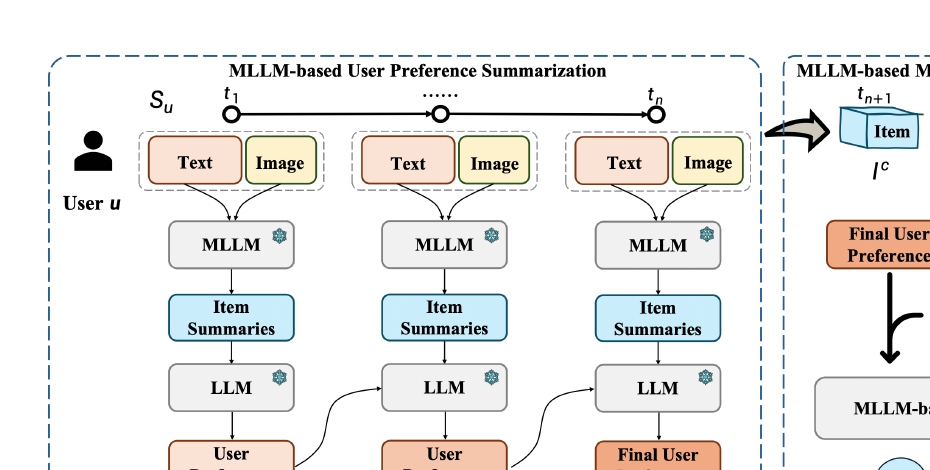
\includegraphics[width=0.78\textwidth]{paper_framework.png}
  \vspace{0.08cm}\scriptsize
  \textbf{Stage 1:} item text/image $\rightarrow$ item summaries $\rightarrow$ recurrent user preference.\quad
  \textbf{Stage 2:} final preference + candidate text/image $\rightarrow$ MLLM recommender $\rightarrow$ yes/no.
\end{frame}

\begin{frame}{Hai stage, hai vai trò của mô hình ngôn ngữ}
  \begin{columns}[T,onlytextwidth]
    \begin{column}{0.47\textwidth}
      \begin{block}{Multimodal User Preferences Inference}
        \begin{enumerate}
          \item MLLM tóm tắt thông tin từng item.
          \item LLM cập nhật preference theo từng block.
          \item Output là văn bản giàu ngữ nghĩa, có thể đọc/giải thích.
        \end{enumerate}
      \end{block}
    \end{column}
    \begin{column}{0.47\textwidth}
      \begin{block}{Tuning MLLM-based Recommender}
        \begin{enumerate}
          \item Đưa preference, item text và image vào prompt.
          \item SFT trên interaction labels.
          \item Chỉ sinh `yes` hoặc `no`; lấy xác suất token đầu tiên.
        \end{enumerate}
      \end{block}
    \end{column}
  \end{columns}
\end{frame}

\subsection{Item summarization}
\begin{frame}{Stage 1 — Tóm tắt item đa phương thức}
  \begin{columns}[T,onlytextwidth]
    \begin{column}{0.34\textwidth}\centering
      \begin{tikzpicture}[node distance=0.35cm, every node/.style={font=\scriptsize}]
        \node[draw,rounded corners,fill=blue!12] (t) {Title / text};
        \node[draw,rounded corners,fill=green!12,below=of t] (i) {Image};
        \node[draw,rounded corners,fill=orange!20,right=1cm of t] (m) {MLLM};
        \node[draw,rounded corners,fill=cyan!15,right=1cm of m] (s) {Item summary};
        \draw[-{Latex}] (t)--(m);\draw[-{Latex}] (i)--(m);\draw[-{Latex}] (m)--(s);
      \end{tikzpicture}
    \end{column}
    \begin{column}{0.59\textwidth}\small
      \begin{enumerate}
        \item Xử lý text summary và image description bằng prompt riêng để khai thác đủ từng modality.
        \item Cân chỉnh độ dài output để text không lấn át image description.
        \item Dùng fusion prompt để hợp nhất thành một mô tả item bằng ngôn ngữ.
      \end{enumerate}
      \begin{block}{\scriptsize Ý nghĩa thiết kế}
        \scriptsize
        Biến bài toán “nhiều image theo thứ tự” thành “chuỗi mô tả item”, phù hợp với năng lực xử lý text dài của LLM.
      \end{block}
    \end{column}
  \end{columns}
\end{frame}

\begin{frame}{Preliminary study: image summary có giữ được tín hiệu?}
  \small Paper dùng GRU4Rec để so sánh input là image summary của LLaVA với feature VGG19.
  \begin{table}\centering
    \begin{tabular}{lccc}\toprule
      Input & MicroLens & Amazon-Baby & Amazon-Game\\\midrule
      Image Summary & \textbf{0.7281} & \textbf{0.7318} & 0.7451\\
      VGG19 Features & 0.7154 & 0.7383 & \textbf{0.7532}\\\bottomrule
    \end{tabular}
    \caption{AUC của GRU4Rec với hai loại input \cite{ye2025mllmmsr}.}
  \end{table}
  \vspace{0.2cm}\begin{block}{Kết luận thận trọng}
    Image-to-text summary bảo toàn đủ semantic signal để cạnh tranh với feature trực tiếp ở preliminary study; đây là bằng chứng động lực, không phải chứng minh lossless.
  \end{block}
\end{frame}

\subsection{Recurrent user preference}
\begin{frame}{Stage 2 — Preference như một trạng thái recurrent}
  \begin{columns}[T,onlytextwidth]
    \begin{column}{0.56\textwidth}\centering
      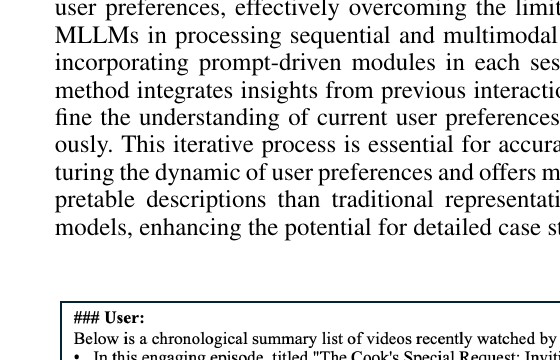
\includegraphics[width=0.98\textwidth]{recurrent_preference.png}
    \end{column}
    \begin{column}{0.4\textwidth}\small
      Chia lịch sử thành các block có thứ tự:
      \begin{equation*}
        \begin{aligned}
          h_k&=\mathrm{LLM}(\mathrm{summary}(B_k),h_{k-1}),\\[-0.1cm]
          h_0&=\varnothing.
        \end{aligned}
      \end{equation*}
      \begin{itemize}
        \item Block đầu tạo preference ban đầu.
        \item Block sau đọc preference trước đó và cập nhật.
        \item $h_k$ là văn bản, nên dễ inspect hơn embedding ẩn.
      \end{itemize}
    \end{column}
  \end{columns}
\end{frame}

\begin{frame}{Một vòng cập nhật preference diễn ra thế nào?}
  \begin{enumerate}
    \item Lấy 3 item liên tiếp (paper chọn block size 3 trong implementation).
    \item Mỗi item đã có title + visual description + item summary.
    \item Prompt yêu cầu LLM chỉ tóm tắt sở thích, không lặp lại chi tiết item.
    \item Kết quả trở thành context cho block kế tiếp.
  \end{enumerate}
  \vspace{0.25cm}\begin{block}{Trade-off}
    Block nhỏ: cập nhật thường xuyên nhưng nhiều lần gọi model. Block lớn: ít call hơn nhưng prompt dài, dễ làm mờ sự thay đổi theo thời gian.
  \end{block}
\end{frame}

\section{MLLM recommender và fine-tuning}
\begin{frame}{Từ preference đến quyết định yes/no}
  \centering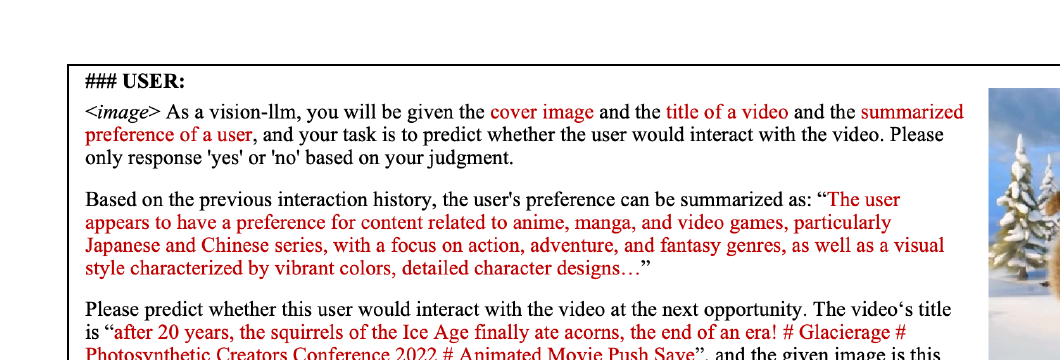
\includegraphics[width=0.94\textwidth]{recommender_training.png}
  \vspace{0.1cm}\small
  Prompt gồm: user preference cuối cùng + lịch sử cần thiết + title candidate + cover image candidate. MLLM được yêu cầu chỉ sinh một nhãn `YES` hoặc `NO` để loại bỏ phần giải thích ngoài ý muốn.
\end{frame}

\begin{frame}{Xác suất tương tác từ token đầu tiên}
  \begin{columns}[T,onlytextwidth]
    \begin{column}{0.55\textwidth}
      Với hai token đầu ra `yes` và `no`, paper định nghĩa:
      \begin{equation}\tag{1}
        p=\frac{p(\text{yes})}{p(\text{yes})+p(\text{no})}.
      \end{equation}
      \small Đây là điểm liên tục để phân loại hoặc xếp hạng candidate, dù visible output chỉ là yes/no.
    \end{column}
    \begin{column}{0.38\textwidth}
      \begin{block}{Điểm đáng chú ý}
        Không thiết kế ranking head riêng. Paper tận dụng next-token probability của MLLM sau khi đã đưa modality và preference vào prompt.
      \end{block}
    \end{column}
  \end{columns}
\end{frame}

\begin{frame}{SFT objective và LoRA}
  \begin{equation}
    \mathcal{L}=-\sum_{i=1}^{L}\log P(v_i\mid v_{<i},\mathcal{I}).
  \end{equation}
  \begin{itemize}
    \item $v_i$: token thứ $i$ của prompt/target sequence; $\mathcal{I}$: image candidate.
    \item Positive/negative interactions tạo supervision cho đáp án yes/no.
    \item LoRA cập nhật ma trận hạng thấp thay vì toàn bộ trọng số MLLM — giảm chi phí fine-tuning và nguy cơ overfit.
  \end{itemize}
  \vspace{0.2cm}\begin{block}{Cấu hình paper}
    LLaVA-v1.6-Mistral-7B; Llama-3-8B-Instruct cho preference summarization; LoRA rank 8, AdamW learning rate $2\times10^{-5}$, batch size 1, gradient accumulation 8, 10 epochs, max length 512.
  \end{block}
\end{frame}

\begin{frame}{Negative sampling và protocol học}
  \begin{tikzpicture}[node distance=0.55cm, every node/.style={font=\small}]
    \node[draw,rounded corners,fill=green!15,minimum width=2.2cm] (p) {Positive item};
    \node[draw,rounded corners,fill=red!12,below=of p,minimum width=2.2cm] (n) {Negative items};
    \node[draw,rounded corners,fill=orange!18,right=1.3cm of p,minimum width=3cm] (q) {Preference + item + image};
    \node[draw,rounded corners,fill=blue!12,right=1.3cm of q,minimum width=2.4cm] (o) {YES / NO};
    \draw[-{Latex}] (p)--(q);\draw[-{Latex}] (n)--(q);\draw[-{Latex}] (q)--(o);
  \end{tikzpicture}
  \vspace{0.35cm}\small
  \scriptsize Training dùng tỷ lệ positive:negative = 1:1; evaluation dùng 1:20. Candidate set được chuẩn hóa để so sánh công bằng giữa các baseline.
\end{frame}

\section{Đối chiếu với implementation trong repo}
\begin{frame}{Paper \texorpdfstring{$\leftrightarrow$}{<->} code repo}
  \begin{table}\centering\tiny
    \begin{tabular}{p{2.9cm}p{6.9cm}}\toprule
      \textbf{Khối trong paper} & \textbf{File trong repo}\\\midrule
      Item image summary & \texttt{Inference/microlens/}\texttt{image\_summary.py} — tạo mô tả ảnh bằng LLaVA; đã verify file tồn tại.\\
      Recurrent preference & \texttt{Inference/microlens/}\texttt{preferece\_inference\_recurrent.py} — chunk 3 item, cập nhật summary bằng Llama 3; đã verify file tồn tại.\\
      Dataset construction & \texttt{train/microlens/}\texttt{dataset\_create.py}, \texttt{test/microlens/}\texttt{multi\_col\_dataset.py}; đã verify file tồn tại.\\
      MLLM SFT & \texttt{train/microlens/}\texttt{train\_llava\_sft.py} — LLaVA + LoRA + PyTorch Lightning; đã verify file tồn tại.\\
      Evaluation & \texttt{test/microlens/}\texttt{test\_with\_llava\_sft.py}; đã verify file tồn tại.\\\bottomrule
    \end{tabular}
  \end{table}
  \vspace{0.15cm}\scriptsize\textcolor{Logo1}{Lưu ý:} đây là đối chiếu implementation trong repo, không thay thế thông số được báo cáo trong paper.
\end{frame}

\begin{frame}{Một số sai khác cần ghi nhớ khi tái hiện}
  \begin{itemize}
    \item \textbf{Đã verify trực tiếp tại `train/microlens/train\_llava\_sft.py`:} paper báo cáo LoRA rank 8, 10 epochs và max length 512; checkout hiện tại đặt `LORA\_R=16`, `EPOCH=4`, `MAX\_LENGTH=1024` (dòng 1--4).
    \item \textbf{Đã verify trực tiếp trong checkout hiện tại:} paper dùng Amazon-Baby/Amazon-Game; repo có các file xử lý `data/amazon/processed/Baby\_Products\_*` và `Video\_Games\_*`, không dùng đúng tên thư mục dataset của paper.
    \item `accumulate\_grad\_batches=4` trong repo hiện tại (dòng 242--248), trong khi paper báo cáo gradient accumulation 8; đây là khác biệt cấu hình cần giữ riêng.
    \item README có một số đường dẫn script cũ; khi chạy cần dùng path thực tế dưới \texttt{MLLM-MSR/train}, \texttt{MLLM-MSR/test} và \texttt{Inference/microlens}.
  \end{itemize}
  \begin{block}{Bài học tái lập}
    Phải phân biệt “con số trong paper” với “cấu hình của code checkout hiện tại”; nếu không, kết quả chạy lại không nhất thiết khớp bảng báo cáo.
  \end{block}
\end{frame}

\section{Thực nghiệm}
\begin{frame}{Datasets và thống kê}
  \begin{table}\centering\scriptsize
    \begin{tabular}{lrrr}\toprule
      & MicroLens & Amazon-Baby & Amazon-Game\\\midrule
      User & 25,411 & 41,081 & 38,808\\
      Item & 20,276 & 14,393 & 13,379\\
      Interaction & 223,263 & 400,876 & 352,136\\
      Avg. sequence length & 11.35 & 13.65 & 13.23\\
      Sparsity & 99.96\% & 99.93\% & 99.93\%\\\bottomrule
    \end{tabular}
    \caption{Thống kê dataset theo paper \cite{ye2025mllmmsr}.}
  \end{table}
  \begin{itemize}\small
    \item MicroLens: user–video interaction, video introduction và cover image.
    \item Amazon: user–product interaction, product description và product image.
    \item Loại user/item quá ít tương tác để bảo đảm history có độ dài tối thiểu.
  \end{itemize}
\end{frame}

\begin{frame}{Baseline và metrics}
  \begin{columns}[T,onlytextwidth]
    \begin{column}{0.46\textwidth}\small
      \textbf{Nhóm baseline}
      \begin{itemize}
        \item Basic SR: GRU4Rec, SASRec.
        \item Multimodal: MGAT, MMGCN.
        \item Multimodal-enhanced SR: GRU4RecF, SASRecF, MMSR, Trans2D.
        \item LLM-based: LLaVA w/o SFT, TALLREC.
      \end{itemize}
    \end{column}
    \begin{column}{0.46\textwidth}\small
      \textbf{Metrics}
      \begin{itemize}
        \item AUC: chất lượng phân biệt positive/negative.
        \item HR@5: hit rate trong top 5.
        \item MRR@5: vị trí của item đúng trong top 5.
      \end{itemize}
      \vspace{0.1cm}Paper dùng 5-fold cross-validation, nhiều random seeds và báo cáo confidence level 95\%.
    \end{column}
  \end{columns}
\end{frame}


\section{Kết quả và phân tích}
\begin{frame}{Kết quả chính — MLLM-MSR dẫn đầu ở cả classification và ranking}
  \begin{table}\centering\tiny
    \begin{tabular}{lccc|ccc|ccc}\toprule
      & \multicolumn{3}{c|}{MicroLens} & \multicolumn{3}{c|}{Video-Games} & \multicolumn{3}{c}{Amazon-Baby}\\
      Model & AUC & HR@5 & MRR@5 & AUC & HR@5 & MRR@5 & AUC & HR@5 & MRR@5\\\midrule
      LLaVA & 52.75 & 28.21 & 17.33 & 53.57 & 33.24 & 18.73 & 55.86 & 34.82 & 20.96\\
      TALLREC & 81.25 & 71.23 & 58.22 & 81.79 & 72.36 & 57.38 & 82.16 & 74.31 & 60.15\\
      \textbf{MLLM-MSR} & \textbf{83.17} & \textbf{78.23} & \textbf{60.38} & \textbf{84.39} & \textbf{77.42} & \textbf{63.25} & \textbf{85.69} & \textbf{79.58} & \textbf{63.77}\\\bottomrule
    \end{tabular}
    \caption{Trích các baseline quan trọng từ Table 3 của paper \cite{ye2025mllmmsr}.}
  \end{table}
  \vspace{0.15cm}\small
  \begin{itemize}
    \item So với TALLREC, MLLM-MSR thêm image signal và preference inference recurrent.
    \item So với LLaVA chưa fine-tune, task-specific SFT là khác biệt rất lớn.
  \end{itemize}
\end{frame}

\begin{frame}{Đọc kết quả theo từng nhóm baseline}
  \begin{enumerate}
    \item \textbf{SR cơ bản:} có sequence nhưng thiếu rich multimodal context.
    \item \textbf{Multimodal graph:} có image/text nhưng không mô hình hóa temporal dynamics đủ mạnh.
    \item \textbf{LLM text-only:} hiểu semantic tốt nhưng không nhìn thấy visual style.
    \item \textbf{MLLM-MSR:} kết hợp cả ba năng lực — modality fusion, sequence modeling và task-specific tuning.
  \end{enumerate}
  \vspace{0.25cm}\centering\large\textcolor{Logo1}{Điểm mạnh không đến từ một module đơn lẻ, mà từ sự ghép đúng các inductive bias.}
\end{frame}


\begin{frame}{Ablation: bỏ một thành phần thì chuyện gì xảy ra?}
  \begin{columns}[T,onlytextwidth]
    \begin{column}{0.5\textwidth}\centering
      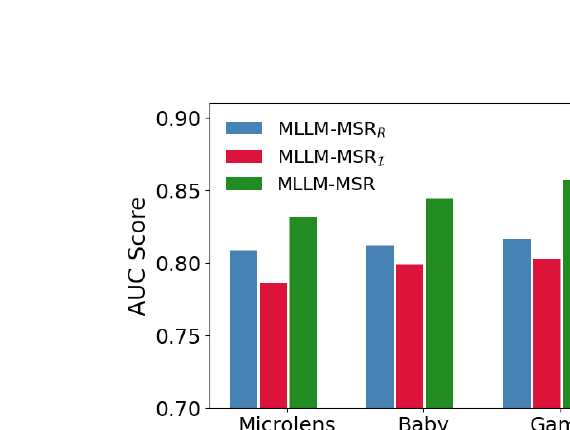
\includegraphics[width=\textwidth]{ablation_variants.png}
    \end{column}
    \begin{column}{0.45\textwidth}\small
      \textbf{MLLM-MSR\textsubscript{R}} — direct inference trên toàn bộ history:
      \begin{itemize}\item prompt dài hơn;\item bỏ qua cập nhật state theo block;\item AUC thấp hơn model đầy đủ.\end{itemize}
      \textbf{MLLM-MSR\textsubscript{I}} — bỏ image summarization:
      \begin{itemize}\item preference inference chỉ còn text;\item mất visual style;\item kết quả giảm dù recommender vẫn nhận image candidate.\end{itemize}
    \end{column}
  \end{columns}
  \vspace{0.05cm}\scriptsize\textcolor{Logo1}{Hình được crop trực tiếp từ Figure 4 của paper; phần chữ bên phải diễn giải đúng mô tả ablation của tác giả.}
\end{frame}

\begin{frame}{Parameter analysis: block size và context length}
  \begin{columns}[T,onlytextwidth]
    \begin{column}{0.47\textwidth}\centering\small
      \textbf{Block size}\par\vspace{0.1cm}
      \resizebox{0.96\linewidth}{!}{\begin{tikzpicture}[x=0.7cm,y=1.8cm]
        \draw[->] (0,0)--(5.3,0) node[right,font=\scriptsize]{block};
        \draw[->] (0,0)--(0,1.1) node[above,font=\scriptsize]{AUC};
        \draw[Logo1,thick] (0.4,0.35)--(1.4,0.65)--(2.4,0.82)--(3.4,0.79)--(4.4,0.58);
        \foreach \x/\v in {0.4/0.35,1.4/0.65,2.4/0.82,3.4/0.79,4.4/0.58} {\fill[Logo1] (\x,\v) circle (1.5pt);}
        \node[font=\scriptsize,align=center] at (2.5,-0.18) {nhỏ: thiếu context\\lớn: prompt dài};
      \end{tikzpicture}}
    \end{column}
    \begin{column}{0.47\textwidth}\centering\small
      \textbf{Preference summary length}\par\vspace{0.1cm}
      \resizebox{0.96\linewidth}{!}{\begin{tikzpicture}[x=0.7cm,y=1.8cm]
        \draw[->] (0,0)--(5.3,0) node[right,font=\scriptsize]{context};
        \draw[->] (0,0)--(0,1.1) node[above,font=\scriptsize]{metric};
        \draw[Logo2,thick] plot coordinates {(0.4,0.25)(1.4,0.48)(2.4,0.78)(3.4,0.8)(4.4,0.8)};
        \foreach \x/\v in {0.4/0.25,1.4/0.48,2.4/0.78,3.4/0.8,4.4/0.8} {\fill[Logo2] (\x,\v) circle (1.5pt);}
        \node[font=\scriptsize,align=center] at (2.5,-0.18) {ngắn: mất thông tin\\đủ dài: ổn định};
      \end{tikzpicture}}
    \end{column}
  \end{columns}
  \vspace{0.15cm}\scriptsize Các đường cong là sơ đồ diễn giải xu hướng trong Figure 5–6 của paper, không phải số liệu tái vẽ chính xác.
\end{frame}

\begin{frame}{Qualitative case: preference summary giúp giải thích dự đoán}
  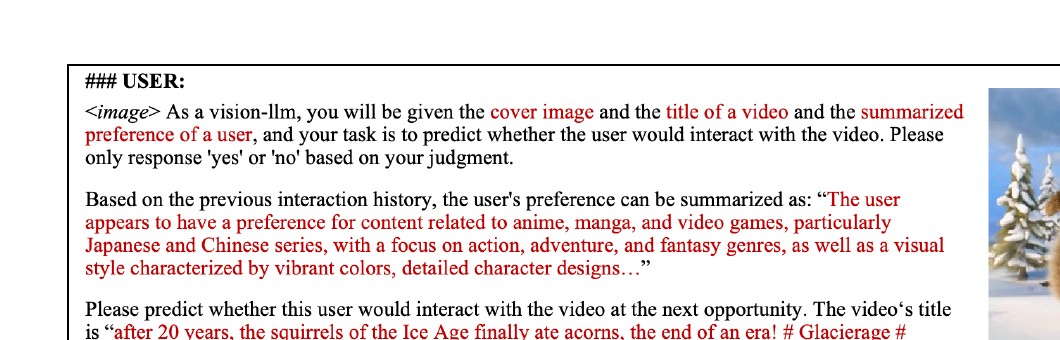
\includegraphics[width=0.96\textwidth]{qualitative_case_01.png}
  \par\vspace{0.1cm}\scriptsize
  Ví dụ trong paper: preference tóm tắt được anime/manga/game, phong cách Nhật–Trung, màu sắc sống động và thiết kế nhân vật chi tiết; candidate có cover hoạt hình được dự đoán `YES`.
\end{frame}

\section{Phê bình và giới hạn}
\begin{frame}{Điều paper làm tốt}
  \begin{itemize}
    \item Đặt đúng giao điểm của ba vấn đề: đa phương thức, tuần tự và MLLM.
    \item Chuyển image thành text để giải quyết context dài bằng một cơ chế đơn giản, dễ triển khai.
    \item Recurrent prompt tạo ra intermediate preference có thể đọc và phân tích.
    \item So sánh đa dataset, nhiều nhóm baseline, có ablation và parameter analysis.
  \end{itemize}
\end{frame}

\begin{frame}{Các giới hạn cần hỏi thêm}
  \begin{itemize}
    \item \textbf{Information bottleneck:} mọi visual cue cuối cùng bị nén qua generated text summary.
    \item \textbf{Chi phí inference:} mỗi block cần gọi LLM; history dài làm tăng số lần gọi và độ trễ.
    \item \textbf{Evaluation gap:} paper chứng minh offline metrics, chưa chứng minh latency, cost hoặc online user satisfaction.
    \item \textbf{Reproducibility gap:} code checkout hiện tại có hyperparameter khác paper, nên cần log rõ cấu hình để tái hiện.
    \item \textbf{Calibration:} xác suất yes/(yes+no) phụ thuộc tokenization và calibration của MLLM, chưa phải xác suất tương tác tuyệt đối.
  \end{itemize}
\end{frame}


\section{Kết luận}
\begin{frame}{Ba thông điệp cần nhớ}
  \begin{enumerate}
    \item \textbf{Chuẩn hóa đa phương thức thành ngôn ngữ:} MLLM biến ảnh + text của từng item thành mô tả hợp nhất, dễ đưa vào chuỗi dài.
    \item \textbf{Preference là trạng thái động:} recurrent summarization cập nhật sở thích qua từng block, thay vì ném toàn bộ lịch sử vào một prompt.
    \item \textbf{MLLM cần được huấn luyện đúng nhiệm vụ:} SFT + LoRA biến LLaVA thành bộ dự đoán yes/no cho candidate item.
  \end{enumerate}
  \vspace{0.3cm}\centering\Large\textcolor{Logo1}{Multimodal + Sequential + Interpretable}
\end{frame}
\begin{frame}{Câu hỏi thảo luận với giảng viên}
  \begin{enumerate}
    \item Image-to-text có làm mất tín hiệu thị giác nào quan trọng cho recommendation không?
    \item Có thể giữ trực tiếp image token nhưng vẫn kiểm soát được chuỗi lịch sử dài bằng memory/attention hiệu quả hơn không?
    \item Điểm số yes/no có đủ để xếp hạng hàng nghìn candidate item trong production không?
    \item Làm thế nào đánh giá chất lượng của preference summary độc lập với recommendation metric?
  \end{enumerate}
\end{frame}
\begin{frame}[allowframebreaks]{Tài liệu tham khảo}\tiny\bibliographystyle{ieeetr}\bibliography{ref/ref}\end{frame}
\end{document}
